\documentclass[tikz,border=10pt]{standalone}
\usepackage{amsmath}
\begin{document}
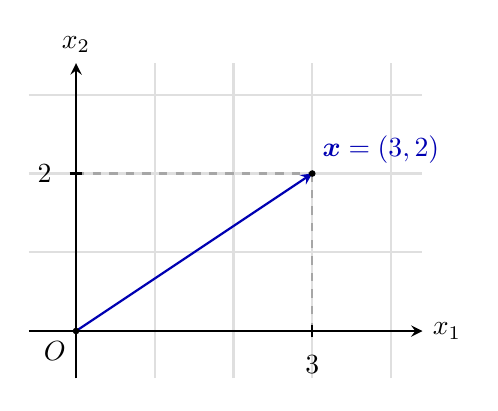
\begin{tikzpicture}[scale=1, >=stealth, line width=0.8pt]
  % Cuadrícula
  \draw[gray!25, step=1cm] (-0.6,-0.6) grid (4.4,3.4);
  % Ejes
  \draw[->] (-0.6,0) -- (4.4,0) node[right] {$x_1$};
  \draw[->] (0,-0.6) -- (0,3.4) node[above] {$x_2$};
  % Líneas auxiliares hasta el punto (3,2)
  \draw[dashed, gray!70] (3,0) -- (3,2);
  \draw[dashed, gray!70] (0,2) -- (3,2);
  % Marcas de coordenadas en los ejes
  \draw (3,-0.08) -- (3,0.08);
  \node[below] at (3,-0.18) {$3$};
  \draw (-0.08,2) -- (0.08,2);
  \node[left] at (-0.18,2) {$2$};
  % Vector x
  \draw[->, thick, blue!70!black] (0,0) -- (3,2) node[above right] {$\boldsymbol{x}=(3,2)$};
  % Origen y punto
  \fill (0,0) circle (1.2pt) node[below left] {$O$};
  \fill (3,2) circle (1.2pt);
\end{tikzpicture}
\end{document}
